\documentclass[12pt]{article}
\usepackage{amsmath}
\usepackage{listings}
\usepackage{amsfonts}
\usepackage{graphicx}
\graphicspath{ {img/} }
\newenvironment{definition}[1][Formal Definition]{\begin{trivlist}\item[\hskip \labelsep {\bfseries #1}]}{\end{trivlist}}
\newenvironment{indef}[1][Informal Definition]{\begin{trivlist}\item[\hskip \labelsep {\bfseries #1}]}{\end{trivlist}} 

\title{Machine Learning Algorithms Illustrated in Python}
\author{Cameron P. Dart}

\begin{document}
\lstset{
	language=Python,
	numbers=left,
    breaklines=true,
    tabsize=2,
    literate={\ \ }{{\ }}1	
}
\maketitle

% Abstract
\begin{abstract}
In order to gain a deeper understanding of \textit{artificial intelligence} algorithms I will explore a \textit{supervised} learning algorithm, \textit{linear regression}, and an \textit{unsupervised} learning algorithm, \textit{K-means clustering}. After researching these algorithms mathematical descriptions, I will write implementations of each algorithm in Python and visualize their outcomes.
\end{abstract}
% Intro
\section{Introduction}
In this paper, I will strictly define a subset of artificial intelligence called \textit{machine learning}. Before diving into the mathematical and definitions of these algorithms, I will distinguish \textit{supervised} from \textit{unsupervised}. The \textit{supervised} learning algorithm I will explore is known as a \textit{linear regression} and the \textit{unsupervised} learning algorithm is \textit{K-means clustering}.\\ \\
 Additionally, \textit{supervised learning algorithms} are computationally intensive, so before writing any code it would be most useful to compute the algorithm by hand with a \textit{training set}. Doing this will allow me to understand where inefficiencies in code and computation can occur, or what mathematical concepts and definitions I can apply to my code. Once I have my mathematical descriptions written, I will proceed to writing my own code. The popular scientific computing Python library called \textit{NumPy} \cite{NumPy} will be used to to handle most of the heavy computational aspects of these algorithms; and the Python graphing library called \textit{matplotlib} \cite{matplotlib} is used for the visualization of my calculations. 
% Machine Learning
\section{Machine Learning}
Machine learning is one of the many subsets of \textit{artificial intelligence}, or the study of how to make computers capable of intelligent behavior. Specifically, it deals with the creation of data driven algorithms. These are algorithms produce patterns based on given input and use the patterns to predict future cases. The main differentiation of machine learning from another subset of artificial intelligence is that the data drives discovery. For example, say an individual is writing an algorithm that detects what a face looks like. A machine learning algorithm would learn by example, juxtaposed to another type of algorithm that would strictly define what a face looks like inside the code. Inside of machine learning there primarily two different types of algorithms, supervised and unsupervised learning.
% Supervised Learning
\section{Supervised Learning Algorithms}
\subsection{Definition}
In \textit{supervised learning} there are two groups of algorithms: classification and regression that both complete the task of deducing a continuous function from a given \textit{training set}. \cite{Ng} A \textit{training set} is a vector of discrete values used for the initial discovery of relationships between variables. In order to prevent \textit{overfitting}, deducing conclusions when none exist, a \textit{validation set} is used in case any classification parameter needs to be adjusted. Further on, a \textit{test set} is used to gauge the efficiency of a given model. \cite{Ng} One classic example of a \textit{supervised learning} algorithm is a \textit{linear regression}. Going back to our example an algorithm that classifying a face, a supervised learning algorithm would learn through examples what a face looks like in terms of its properties, such as color, structure, and size so it can classify later inputs based on what it previously observed.
\subsection{Example: Linear Regression}
\subsubsection{Definition}
A \textit{linear regression} is an approach for modeling the relationship between a scalar dependent variable $y$ and one or more explanatory variables (or independent variables) denoted $X$. Specifically the case of one explanatory variable is called a \textit{linear regression}. A sample data set for a linear regression would be pairs $(x_1,y_1),(x_2,y_2),....,(x_n,y_n)$ where the regression models $y_i$ as a function of $x_i$
\subsubsection{Mathematical Description}
The \textit{regression line} can be determined by finding \textit{sum of squares} method. A
\textit{fitted linear regression line} can be described as
\begin{equation}
\hat y=\hat \beta_{0}+\hat \beta_1*x \, \, \, \, \, \,\cite{GATech}
\end{equation}
$\hat \beta_0$ is defined as 
\begin{equation}
	\hat \beta_0 = \bar y - \hat \beta_1 \bar x
\end{equation}
Given $n$ is the number of data points in the \textit{training set}\\
\begin{equation}
	\bar y \equiv \frac{1}{n} \sum y_i
\end{equation}
\begin{equation}
	\bar x \equiv \frac{1}{n}\sum x_i	
\end{equation}

\begin{equation}
	\hat \beta_1 = \left(\frac{n \sum x_iy_i - (\sum x_i)(\sum y_i)}{n\sum x_i^2 - (\sum x_i)^2}\right)
\end{equation}
An easier way to express $\hat \beta_1$ can be defined as
\begin{equation}
	\hat \beta_1 = \frac{S_{xy}}{S_{xx}}
\end{equation}
Where $S_{xy}$ and $S_{xx}$ are 
\begin{align*}
S_{xy}&= \sum(x_i-\bar x)(y_i-\bar y) \\
	  &= \sum x_iy_i-\frac{(\sum x_i)(\sum y_i)}{n}\\
	  &= \sum x_iy_i-\bar x *\bar y
\end{align*}

\begin{align*}
S_{xx} &= \sum(x_i - \bar x)^2 \\
&= \sum (x_i)^2 - \frac{(\sum x_i)^2}{n}\\
&= \sum (x_i)^2 - \bar x
\end{align*}

\subsubsection{Example Use Case}
You are given a vector of training data, $V$, such that $V = \left \{(x_1,y_1), ... ,(x_n,y_n) \right \}$ where $x_i$ is the amount of hours an individual studied for a test and $y_i$ is their score on that test. \\
Let the pairs of values of $V$ be defined in the table given below.
\begin{center}
    \begin{tabular}{ | l | l |} \hline
	    X: Time Studied (Hours) & Y: Score (Out of 800)  \\ \hline
		    4 & 390 \\ \hline
			9 & 580 \\ \hline
			10 & 650 \\ \hline
			14 & 730 \\ \hline
			4 & 410 \\ \hline
			7 & 530 \\ \hline
			12 & 600 \\ \hline
			22 & 790 \\ \hline
			1 & 350 \\ \hline
			3 & 400 \\ \hline
			8 & 590 \\ \hline
			11 & 640 \\ \hline
			5 & 450 \\ \hline
			6 & 520 \\ \hline
			10 & 690 \\ \hline
			11 & 690 \\ \hline
			16 & 770 \\ \hline
			13 & 700 \\ \hline
			13 & 730 \\ \hline
			10 & 64 \\ \hline
    \end{tabular}
\end{center}

\subsubsection{Calculations}
First, I will calculate $\bar x$ and $\bar y$, better known as the average values for $x$ and $y$ respectively\\
\begin{align*}
\bar x &= \frac{1}{n} * \sum_{i=1}^{20}x_i\\
&= \frac{1}{20} * \sum_{i=1}^{20}x_i\\
&= \frac{1}{20} * 157\\
&= 8.72\\ \\
\bar y &= \frac{1}{n} * \sum_{i=1}^{20}y_i\\
&= \frac{1}{20} * \sum_{i=1}^{20}y_i\\
&= \frac{1}{20} * 10420\\
&= 578.89\\
\end{align*}
Thus, based on our training set defined above $\bar x = 8.72$ and $\bar y = 578.89$\\
Next, I will use the previous calculations of $\bar x$ and $\bar y$ to calculate $S_{xy}$ and $S_{xx}$
\begin{align*}
S_{xx} &= \sum_{i=1}^{i=20} (x_i)^2 - \bar x \\
&= \sum_{i=1}^{i=20} (x_i)^2 - \sum{i=1}^{i=20} \bar x \\
&= 285.31 \\
S_{xy} &= \sum_{i=1}^{i=20} (x_i)(y_i) - \bar x \bar y \\
&= \sum_{i=1}^{i=20} (x_i)(y_i) - \sum_{i=1}^{i=20} \bar x \bar y \\
&= 8598.02
\end{align*}
Now, we have all calculations we need to find where $\beta_{1}$
\begin{align*}
	\beta_{1} &= \frac{S_{xy}}{S_{xx}} \\
	&= \frac{8598.02}{285.31} \\
	&= 30.14
\end{align*}
Now since we have $\beta_{0}$ we can use it in our final calculation of $\beta_{0}$
\begin{align*}
	\beta_{0} &= \bar y - \beta_{1} * \bar x \\
	&= 578.89 - 8.24 * 9.45 \\
	&= 316.82
\end{align*}
Our linear regression line is now \\
\begin{equation}
	y = 316.04 + 30.14x
\end{equation}
%%%%%%%%%%%%%%%%%%%%%%
\subsubsection{Geometric Representation}
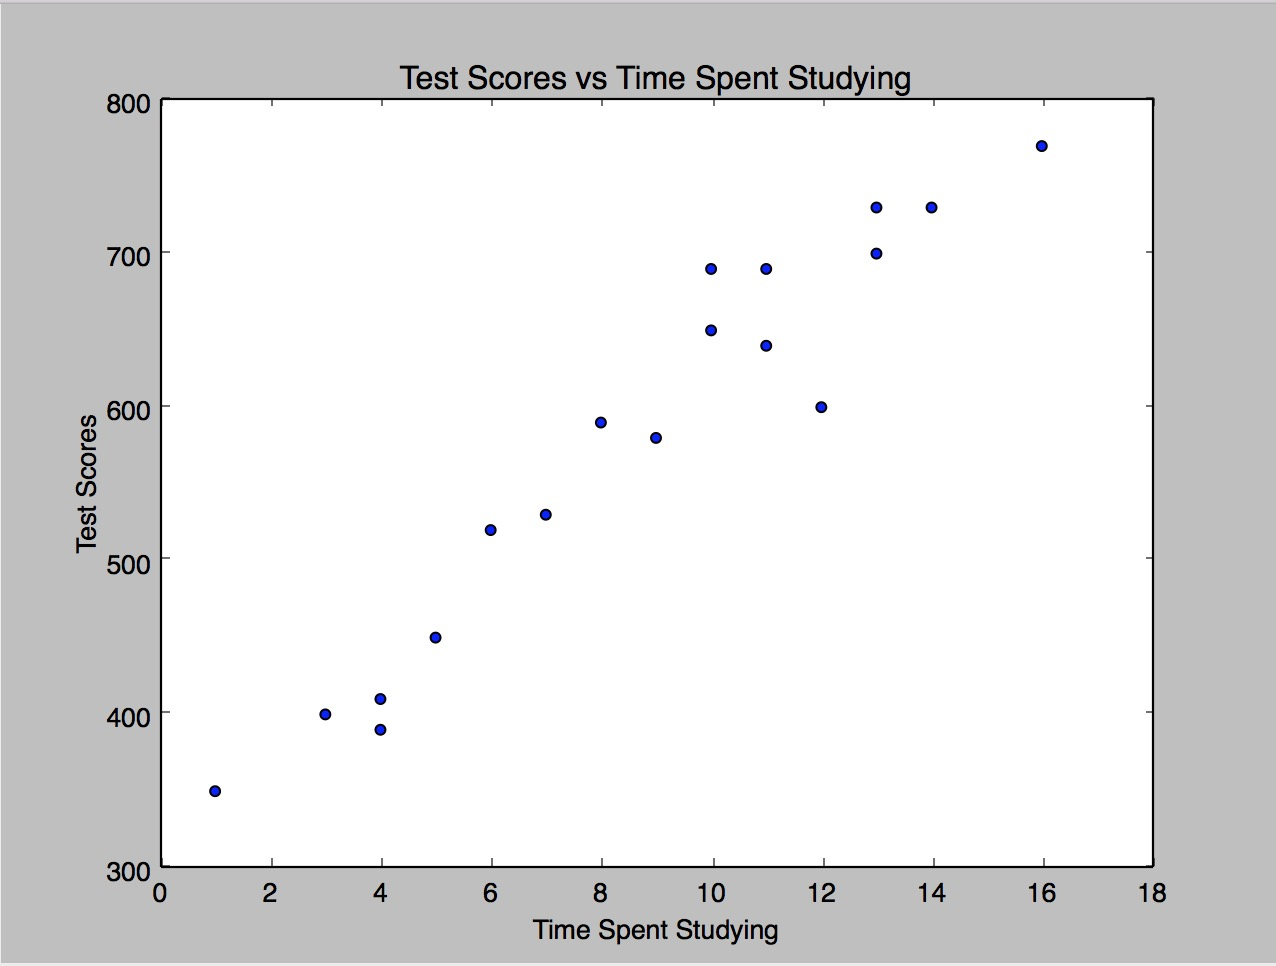
\includegraphics[width=90mm]{img/scatter_plots}
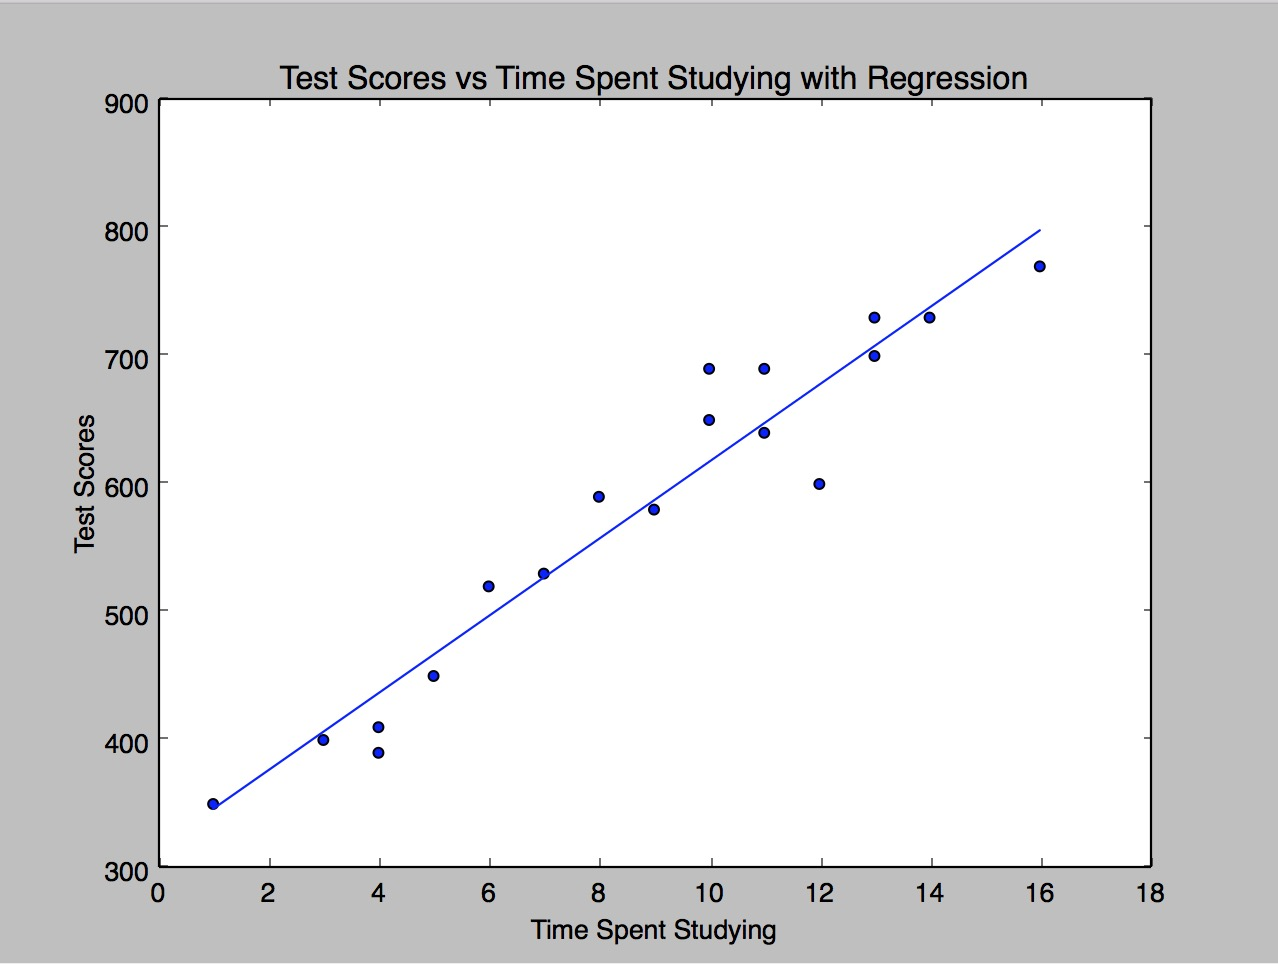
\includegraphics[width=90mm]{img/regression}
As you can see from the two graphs, our linear regression is a strong approximation of our data set. 
%%%%%%%%%%%%%%%%%%%%%%
\subsubsection{Sample Sum of Squares Regression in Python}
\begin{lstlisting}
#!/usr/bin/python
import time # get start and end time of function
import numpy as np # scientific computing library
import matplotlib.pyplot as plt # library to generate plots

class SumSquareRegression:
# Creates instance of SumSquareRegression object	
class SumSquareRegression:
	
	def __init__(self, data_set):

		self.data_set = data_set
		self.avg = self.data_avg(self.data_set)
		self.x_bar = self.avg[0]
		self.y_bar = self.avg[1]
		self.sxxy = self.calculate_sxxy(data_set, self.x_bar, self.y_bar)
		self.sxx = self.sxxy[0]
		self.sxy = self.sxxy[1]
		self.beta_1 = (self.sxy / self.sxx)
		self.beta_0 = (self.y_bar - self.beta_1 * self.x_bar)

	# O(n) time complexity
	# O(1) space complexity
	# Returns an array containing avg x and avg y values
	def data_avg(self, vector):
		sum_x = 0
		sum_y = 0
		size = len(vector) 

		for i in range(0, len(vector) ):
			sum_x += vector[i][0]
			sum_y += vector[i][1]

		# type casting to return a decimal
		return [float(sum_x)/size, float(sum_y)/size]

	# O(n) time complexity
	# O(1) space complexity
	# Returns S_xx and S_yy in an array respectively
	def calculate_sxxy(self, vector, x_bar, y_bar):
		sxx_sum = 0
		sxy_sum = 0

		for i in range(0, len(vector) - 1):
			sxx_sum += (vector[i][0] - self.x_bar) ** 2
			sxy_sum += (vector[i][0] - self.x_bar) * (vector[i][1] - self.y_bar)

		return [sxx_sum, sxy_sum]

	# Prints stats related to regression
	def print_regression_stats(self):
		print "x_bar: %.2f" % self.x_bar
		print "y_bar: %.2f" % self.y_bar
		print "s_xx: %.2f" % self.sxx
		print "s_xy: %.2f" % self.sxy
		print "beta_0: %.2f" % self.beta_0
		print "beta_1: %.2f" % self.beta_1
		print "Regression Line: y = %.2fx + %.2f" % (self.beta_1, self.beta_0)

	def plot_data(self, data):
		x_list = [x for [x, y] in data]
		y_list = [y for [x, y] in data]
		plt.scatter(x_list, y_list)
		plt.ylabel('Test Scores')
		plt.xlabel('Time Spent Studying')
		plt.title('Test Scores vs Time Spent Studying')
		plt.show()

	def plot_with_regression(self, data):
		# plot data
		x_list = [x for [x, y] in data]
		y_list = [y for [x, y] in data]
		plt.scatter(x_list, y_list)
		plt.ylabel('Test Scores')
		plt.xlabel('Time Spent Studying')
		# plot regression
		# uses python list comprehension
		y = [self.regression_approximation(x) for [x, y] in data]
		plt.plot(x_list, y)
		# print plot
		plt.title('Test Scores vs Time Spent Studying with Regression')
		plt.show()		

	def regression_approximation(self, x):
		return (self.beta_1 * x) + (self.beta_0)

# Test Data
def main():
	sample_data_1 = [[4, 390],[9, 580],[10, 650],[14, 730],[4, 410],[7, 530],[12, 600],[1, 350],[3, 400],[8, 590],[11, 640],[5, 450],[6, 520],[10, 690],[11, 690],[16, 770],[13, 700],[13, 730]]
	regression_1 = SumSquareRegression(sample_data_1)
	regression_1.print_regression_stats()
	regression_1.plot_data(sample_data_1)
	regression_1.plot_with_regression(sample_data_1)

# Runs program automatically
if __name__ == '__main__':
	main()
\end{lstlisting}
\section{Unsupervised Learning Algorithms}
\subsection{Definition}
Our expected outcome from unsupervised learning is to derive some structure in the data where none previously existed. That being said, we are "clustering" the data into groups based upon intrinsic relationships found. Hence, this type of algorithm allows user to approach the problem at hand with little to no knowledge of what the result should look like. Back to our example of face classification, an unsupervised algorithm would differentiate faces from cows and dogs, but it would not know, or define, what each group is.  
\subsection{Example K-means clustering}
\subsubsection{Defintion}
Grouping a set of objects into similar subsets is a very common task in data analysis and is often referred to as "clustering". This task can be done in a copious amount of ways, however, one of the most prominent algorithms is \textit{K-means clustering}. The  \textit{K-means clustering} algorithm aims to partition $n \in \mathbb{N}$ points in a $d$ dimensional space into $k > 0$ distinct clusters. Thus, given a vector of data $X \in \mathbb{R}^d$ with $d$ and $n$ given above, our algorithm seeks to find a set $C$ of $k$ centers. \cite{MacKay} 
\subsubsection{Mathematical Description}
Unfortunately, finding solutions to K-means clustering is \textit{NP Hard}. Computational complexity theory describes \textit{NP Hard}  as non-deterministic polynomial time, or it may or may not be able to be solved in polynomial time. \textit{Lloyd's Algorithm} offers an iterative solution to this k-means clustering solution. Let the dataset be a vector $X$ with $n$ points such that $(\forall i \in X)(X_i \in \mathbb{R})$, where $((n>0) \in \mathbb{N})$ as input, given a parameter $((K >0) \in \mathbb{N})$ which determines how many clusters to create. Let the output be a set of $K$ cluster centroids, or centers of data clusters, and a labeling of X that assigns each of the points in X to a unique cluster. All points within a cluster are closer in distance to their centroid than they are to any other centroid. \\
Let $C$ be the set of clusters such that $C_k \subset C$, the set of clusters, $C_k$ be calculated as follows. \\
\begin{equation}
	C_k = \{ x_n : \vert \vert x_n - \mu_k \vert \vert \leq \,\,\, all \,\,\, \vert \vert x_n - \mu_l \vert \vert \}
\end{equation}
$\mu_k$ is defined to be the average values clusters or 
\begin{equation}
\mu_k = \frac{1}{C_k} \sum_{x_n \in C_k} x_n	
\end{equation}

The mathematical condition for the K clusters $C_k$ and the K centroids $\mu_k$ can be expressed as:\\
\begin{equation}
	\text{Minimize} \sum_{k=1}^{K}\,\sum_{x_n \in C_k} (\vert \vert x_n - \mu_k \vert \vert )^2 \text{with respect to}\,\, C_k, \mu_k
\end{equation} \cite{dsl}
The result is a partitioning of a data space into Voronoi cells. This is why \textit{Lloyd's Algorithm} is also called \textit{Voronoi iteration}.
\subsubsection{Example Use Case}
\subsubsection{Sample K-means clustering in Python}
\subsubsection{Geometric Representation}
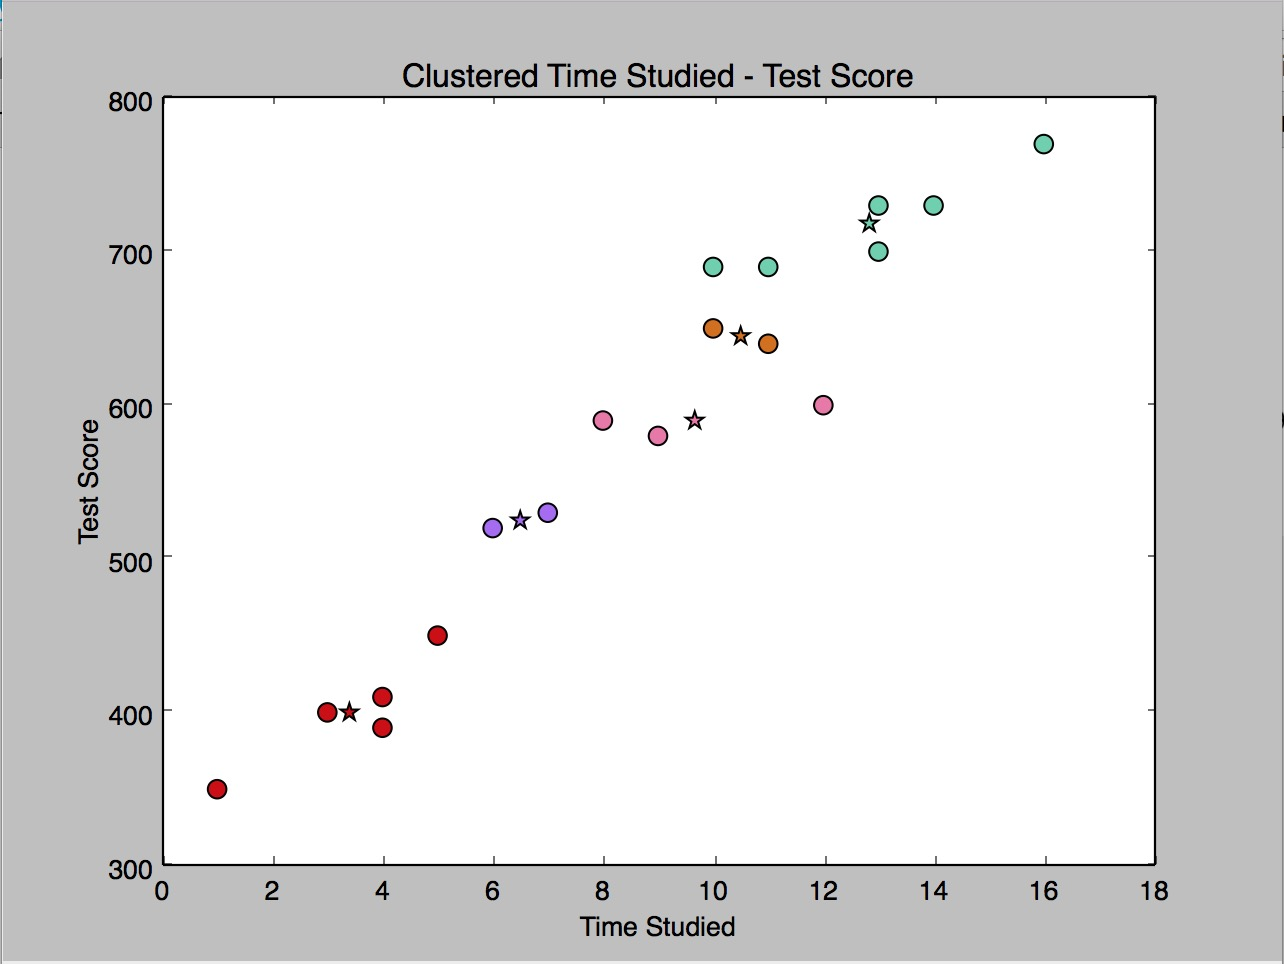
\includegraphics[width=90mm]{img/clustered}\\
\begin{lstlisting}
#!/usr/bin/python
import numpy as np # scientific computing library
import matplotlib.pyplot as plt # plotting
import random # used to generate random centroids

class KMeansClustering:

	def __init__(self, data_set, k):
		self.data_set = data_set
		self.k = k

	# for each point in data set,
	# find new subset it belongs too.
	def generate_clusters(self, mu):
	    clusters  = {}
	    for pt in self.data_set:
    		# for each pt in our data set 
    		# find best fitting value
				best_mu = min([(array[0], np.linalg.norm(pt - mu[array[0]])) \
									for array in enumerate(mu)], key = lambda t:t[1])[0]
				try:
					clusters[best_mu].append(pt)
				except KeyError:
					clusters[best_mu] = [pt]
	    return clusters
	 
	# calcuate new mu values
	def reevaluate_centers(self, mu, clusters):
	    new_mu = []
	    keys = sorted(clusters.keys())
	    for k in keys:
	        new_mu.append(np.mean(clusters[k], axis = 0))
	    return new_mu
	 
	def has_converged(self, mu, old_mu):
			# we know we have converged if our old and new mu values are the same
	    return (set([tuple(a) for a in mu]) == set([tuple(a) for a in old_mu]))
	 
	def k_means(self):
	  # at first, randomize centroids 
		old_mu = random.sample(self.data_set, self.k)
		mu = random.sample(self.data_set, self.k)

		while not self.has_converged(mu, old_mu):
			old_mu = mu
	    
	    # assign pts in data_set to clusters
			clusters = self.generate_clusters(mu)
	    
	    # recalculate centers
			mu = self.reevaluate_centers(old_mu, clusters)

 		return(mu, clusters)

def main():
	# Notice this the same as the last dataset 
	# Instead of predictive modeling we'll use this data to split into
	# distinct ranges (think A, B, C, D, F) in this case
	sample_data_1 = np.array([[4, 390],[9, 580],[10, 650],[14, 730],[4, 410],[7, 530],[12, 600],[1, 350],[3, 400],[8, 590],[11, 640],[5, 450],[6, 520],[10, 690],[11, 690],[16, 770],[13, 700],[13, 730]])
	k = 5 # how many different clusters do we want?
	clustered = KMeansClustering(sample_data_1, k) # initialize object
	data = clustered.k_means()
	
	# parse data to plot
	centroids = data[0]
	clusters = data[1]
	i = 0
	for centroid in centroids:
		c = np.random.rand(3,1)
		s = 70, 
		plt.scatter(centroid[0],centroid[1], s, c, marker = '*')
		data = clusters[i]
		for pt in data:
			plt.scatter(pt[0],pt[1], s ,c)
		i += 1
	plt.xlabel('Time Studied')
	plt.ylabel('Test Score')
	plt.title('Clustered Time Studied - Test Score')
	plt.show()

if __name__ == '__main__':
	main()
\end{lstlisting}


\begin{thebibliography}{9}
\bibitem{matplotlib}http://matplotlib.org/
\bibitem{NumPy}http://www.numpy.org/
\bibitem{GATech}http://www2.isye.gatech.edu/\~sman/courses/6739SimpleLinearRegression.pdf
\bibitem{Ng}http://cs229.stanford.edu/notes/cs229-notes1.pdf
\bibitem{dsl}https://datasciencelab.wordpress.com/2013/12/12/clustering-with-k-means-in-python/
\bibitem{MacKay}Mackay, David J. C. (2002) \emph{Information Theory, Inference \& Learning Algorithms} Cambridge University Press
\bibitem{Github}https://github.com/skamdart
\end{thebibliography}

\section*{Acknowledgement}
Source code for this .tex file and my algorithms can be found at my GitHub \cite{Github}
\end{document}